\begin{frame}{\only<1>{\'Expérimentation}}
\begin{center}
\begin{tikzpicture}[mystyle]
\matrix [column sep=10mm,row sep=5mm,ampersand replacement=\&]
{
\& \node (i4) {Exp};  \& \\
\node (i1) {$X$}; \&
\node [terminal] (i2) {$p$}; \&
\node  (i3) {$Y$}; \\
};
\node (box) [draw, line width=1pt, rounded corners, fit =  (i1) (i4) (i3)] {};
\begin{scope}[every path/.style=line]
  \path (i1) -- node [left] {} (i2);
  \path (i2) -- node [right] {} (i3);
\end{scope}
\end{tikzpicture}
\end{center}
\vspace{.8cm}
\only<1>{
\begin{description}
\item[$p$]: processus, traitement, prédicteur
\item[$X$]: entrée, signal, observation
\item[$Y$]: sortie, prédiction
\item[Exp]: protocole expérimental
\end{description}}
\end{frame}


\begin{frame}{Recherche d'information (IR)}
\begin{center}
\begin{tikzpicture}[mystyle]
\matrix [column sep=10mm,row sep=5mm,ampersand replacement=\&]
{
\node (i1) {$X$}; \&
\node [terminal] (i2) {$p$}; \&
\node (i3) {\alert{$y$}}; \\
};
\begin{scope}[every path/.style=line]
  \path (i1) -- node [left] {} (i2);
  \path (i2) -- node [left] {} (i3);
\end{scope}
\end{tikzpicture}
\end{center}
\vspace{.8cm}
\begin{description}
\item[$X$]: données observées (en grande dimension)
\item[$y$]: labels (en petite dimension)
\end{description}
\end{frame}

\begin{frame}{Tâche: recherche d'information (IR)}
\begin{center}
\begin{tikzpicture}[mystyle]
\matrix [column sep=10mm,row sep=5mm,ampersand replacement=\&]
{
\node (i1) {$X$}; \&
\node [terminal] (i2) {$P$}; \&
\node [terminal] (i3) {$C$}; \&
\node (i4) {\alert<1>{$y$}}; \\
};
\begin{scope}[every path/.style=line]
  \path (i1) -- node [left] {} (i2);
\path (i2) -- node [above] {$L$} (i3); \path (i3) -- node [right] {} (i4);
\end{scope}
\end{tikzpicture}
\end{center}
\vspace{.8cm}
\begin{description}
\item[$L$] représentation de $X$ dans un espace latent
\item[but]: $X_j=D(X_i)$, $L_j=d(L_i) \text{ ssi } y_j=y_i$
\item[$D$]: grande déformation
\item[$d$]: petite déformation
\end{description}
\end{frame}

\begin{frame}{Propriétés de $L$}
  \begin{center}
  \begin{tikzpicture}[mystyle]
  \matrix [column sep=10mm,row sep=5mm,ampersand replacement=\&]
  {
  \node (i1) {$X$}; \&
  \node [terminal] (i2) {$P$}; \&
  \node [terminal] (i3) {$C$}; \&
  \node (i4) {\alert<1>{$y$}}; \\
  };
  \begin{scope}[every path/.style=line]
    \path (i1) -- node [left] {} (i2);
  \path (i2) -- node [above] {$L$} (i3); \path (i3) -- node [right] {} (i4);
  \end{scope}
  \end{tikzpicture}
  \end{center}
  \vspace{.8cm}
  \begin{block}{Guidé par les données $X$}
    \begin{itemize}
    \item invariance: translation, ...
    \item stabilité: étirement, ...
    \end{itemize}
  \end{block}
  \begin{block}{Guidé par la tâche $y$}
$$ |L_i-L_j| < |L_i-L_k| \text{ ssi } y_i=y_j \forall k | y_k \neq y_i $$
  \end{block}
\end{frame}


\begin{frame}{IR en audio}
\begin{center}
\begin{tikzpicture}[mystyle]
\matrix [column sep=10mm,row sep=5mm,ampersand replacement=\&]
{
\node (i1) {\only<1>{$X$}\only<2>{Son}}; \&
\node [terminal] (i2) {$P$}; \&
\node [terminal] (i3) {$C$}; \&
\node (i4) {\only<1>{$y$}\only<2>{label}}; \\
};
\begin{scope}[every path/.style=line]
  \path (i1) -- node [left] {} (i2);
  \path (i2) -- node [above] {  } (i3);
  \path (i3) -- node [right] {} (i4);
\end{scope}
\end{tikzpicture}
\end{center}
\vspace{.8cm}
\only<2>{
\begin{description}
\item[$P$]: module de \og perception \fg
\begin{itemize}
    \item plusieurs TFCT à résolutions différentes
    \item réseaux convolutionnels profonds
\end{itemize}
\item[$C$]: module de \og cognition \fg
\begin{itemize}
    \item réseaux neuronaux profonds totalement connectés
    \item fusion
\end{itemize}
\end{description}
}
\end{frame}


\begin{frame}{Communautés}
\begin{block}{Music Information Retrieval (MIR)}
\begin{itemize}
\item 2000 - --
\item Compétition: 18 tâches  (Mirex)
\item Conference : 100 articles (Ismir)
\end{itemize}
\end{block}
\begin{block}{Detection and Classification of
Acoustic Scenes and Events (DCASE)}
\begin{itemize}
\item 2013 - --
\item Compétition: 7 tâches
\item Workshop: 50 articles
\end{itemize}
\end{block}
\end{frame}

\begin{frame}{Contributions}
\begin{center}
\begin{tikzpicture}[mystyle]
\matrix [column sep=10mm,row sep=5mm,ampersand replacement=\&]
{
\& \node (i4) {Exp};  \& \\
\node (i1) {Son}; \&
\node [terminal] (i2) {$p$}; \&
\node  (i3) {label}; \\
};
\node (box) [draw, line width=1pt, rounded corners, fit =  (i1) (i4) (i3)] {};
\begin{scope}[every path/.style=line]
  \path (i1) -- node [left] {} (i2);
  \path (i2) -- node [right] {} (i3);
\end{scope}
\end{tikzpicture}
\end{center}
\vspace{.8cm}
\begin{enumerate}
  \item \structure{Son}: plus de contrôle
  \item \structure{label}: plus de maîtrise
  \item \structure{Exp}: plus de formalisation
\end{enumerate}
\end{frame}


\begin{frame}{Compétitions en IR}
\begin{center}
\begin{tikzpicture}[mystyle]
\matrix [column sep=10mm,row sep=5mm,ampersand replacement=\&]
{
\& \node (i4) {Exp};  \& \\
\node (i1) {Son}; \&
\visible<2->{\node [terminal] (i2) {\only<2>{$p_1$}\only<3>{$p_2$}\only<4>{$p_n$}\only<5->{$p$}}; \&
\node  (i3) {label};} \\
};
\node (box) [draw, line width=1pt, rounded corners, fit =  (i1) (i4) (i3)] {};
\visible<2->{
\begin{scope}[every path/.style=line]
  \path (i1) -- node [left] {} (i2);
  \path (i2) -- node [right] {} (i3);
\end{scope}}
\end{tikzpicture}
\end{center}
\vspace{.8cm}
\only<1-4>{
L’organisateur de la compétition
\begin{itemize}
\item prépare les données ainsi qu'une description du problème
\item fournit des méthodes d'évaluation
\item ...
\end{itemize}
}
\only<5->{
\begin{itemize}
\item Alternative à l'approche \og mon outil, mon jeu de données, ma métrique \fg
\item Spécification de l'expérimentation  \og clés en main \fg
\item biais de conception du protocole assumés collectivement
\end{itemize}
}
\end{frame}

\begin{frame}{Compétitions en crise ?}
\begin{itemize}
    \item cauchemard des métriques
    \item \og la fin justifie les moyens \fg
\end{itemize}
\vspace{.8cm}
\begin{center}
\og Faites quelque chose d'intéressant !! \fg \\
\og ... de scientifique !! \fg \\
\hfill \textit{panel DCASE 2018}
\end{center}
\vspace{.8cm}
$\hookrightarrow{}$ placer l'effort sur un questionnement plutôt que sur la démonstration d'un outil
\end{frame}

\begin{frame}{Design de Compétition}
\begin{block}{Organisation d'une tâche DCASE (2013, 2016)}
\begin{itemize}
\item Tâche de détection d'évènements
\item corpus de scènes sonores simulées
\item sons isolés enregistrés
\item contrôle de haut niveau sur la composition de la scène
\end{itemize}
\end{block}\footfullcitenomarkleft{stowellhal-01253912} \footfullcitenomarkleft{mesa}
\end{frame}

\begin{frame}{Approche  \og psychologie expérimentale \fg}
\begin{itemize}
\item formulation d'une hypothèse : le degré de polyphonie impacte les algorithmes de détection d'évènement sonores
\item production de corpus avec un degré variable de polyphonie
\item choix d'un protocole expérimental adapté
\item les algorithmes sont considérés comme des sujets et leurs concepteurs ne sont pas informés de la typologie du corpus
\item analyse des résultats
\end{itemize} \footfullcitenomarkleft{lafayhal-01111381}
\end{frame}

\begin{frame}{Que prédire ?}
\begin{center}
  \begin{tikzpicture}[mystyle]
  \matrix [column sep=10mm,row sep=5mm,ampersand replacement=\&]
  {
  \& \node (i4) {Exp};  \& \\
  \node (i1) {Son}; \&
  \node [terminal] (i2) {p}; \&
  \node  (i3) {\alert{label}}; \\
  };
  \node (box) [draw, line width=1pt, rounded corners, fit =  (i1) (i4) (i3)] {};
  \begin{scope}[every path/.style=line]
    \path (i1) -- node [left] {} (i2);
    \path (i2) -- node [right] {} (i3);
  \end{scope}
  \end{tikzpicture}
\end{center}
\vspace{.8cm}
\begin{itemize}
\item interface riche avec d'autres communautés
\item nécessité d'alignement des vocabulaires et des temporalités
\end{itemize}
\end{frame}

\begin{frame}{Caractérisation des environnements sonores urbains (ANR CENSE)}
\only<1>{
\begin{itemize}
    \item les qualifiants perceptifs de haut niveau comme l'agrément sont corrélés au temps de présence perçu des sources
    \item prédiction de ces valeurs perceptives par des approches neuronales profondes
\end{itemize}
}
\only<2>{
    \begin{center}
    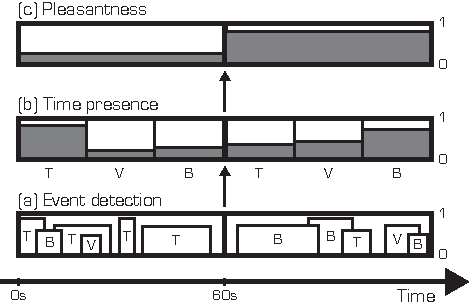
\includegraphics[width=.7\columnwidth]{figures/block}
    \end{center}
}
\footfullcitenomarkleft{gontierActa}
\end{frame}

\begin{frame}{Projet de recherche avec le Conservatoire National de Musique et de Danse de Paris (CNSMDP)}
\begin{itemize}
\item Recherche par similarité dans des corpus de modes de jeux étendus
\item Confrontation d'un modèle computationnel de perception à des jugements experts
\item L'opérateur de diffusion d'ondelettes apporte d'excellents résultats
\end{itemize}
\begin{table}
\small
    \centering
{\footnotesize
\begin{tabular}{c|ccccc}
 joint (1s) + lmnn & -lmnn & (25 ms) &  séparable & mfcc & \\
      \hline
 $96\% \pm 2$ & $93\% \pm 3$ & $91\% \pm 4$ & $91\% \pm 4$ & $82\% \pm 7$ & ($aP@5$)\\
\end{tabular}
}
\end{table}
\footfullcitenomarkleft{lostanlenJasmp}
\end{frame}

\begin{frame}{ExpLanes}
  \begin{center}
    \only<1>{
  \begin{tikzpicture}[mystyle]
  \matrix [column sep=10mm,row sep=5mm,ampersand replacement=\&]
  {
  \& \node (i4) {\alert{Exp}};  \& \\
  \node (i1) {$X$}; \&
  \node [terminal] (i2) {$p$}; \&
  \node  (i3) {$y$}; \\
  };
  \node (box) [draw, line width=1pt, rounded corners, fit =  (i1) (i4) (i3)] {};
  \begin{scope}[every path/.style=line]
    \path (i1) -- node [left] {} (i2);
    \path (i2) -- node [right] {} (i3);
  \end{scope}
\end{tikzpicture}}
\only<2>{  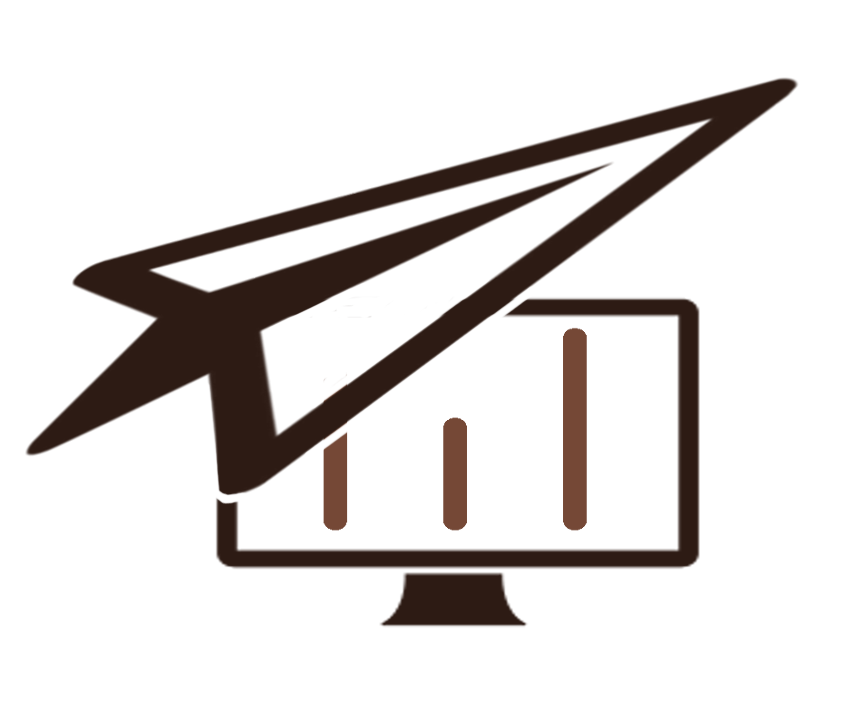
\includegraphics[width=.3\columnwidth]{figures/logoExplanes} \\
   \url{http://mathieulagrange.github.io/expLanes}}
  \end{center}
  \vspace{.8cm}
  \uncover<2>{
ExpLanes, un environnement logiciel qui facilite:
\begin{enumerate}
  \item la gestion des calculs
  \item le traitement des résultats
  \item la reproducibilité
\end{enumerate}
}
\end{frame}

\begin{frame}{ExpLanes}

  \begin{center}
  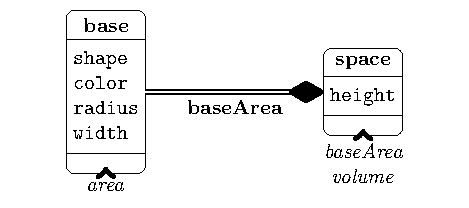
\includegraphics[width=\columnwidth]{figures/factors} \\
  \tiny  \url{https://mathieulagrange.github.io/paperBandwidthExtensionCnn/demo}
  \end{center}
\footfullcitenomarkleft{lagrange2019bandwidth}
\end{frame}

% E
% reproducibilité
% donoho
% protocoles expérimentaux assez canonique
% explanes
% extension de bande
% demonstration
\begin{frame}{Approches étudiées}
\begin{center}
\begin{tikzpicture}[mystyle]
\matrix [column sep=10mm,row sep=5mm,ampersand replacement=\&]
{
\& \node (i4) {\alert{Exp}};  \& \\
\node (i1) {\alert{$X$}}; \&
\node [terminal] (i2) {$p$}; \&
\node  (i3) {\alert{$y$}}; \\
};
\node (box) [draw, line width=1pt, rounded corners, fit =  (i1) (i4) (i3)] {};
\begin{scope}[every path/.style=line]
  \path (i1) -- node [left] {} (i2);
  \path (i2) -- node [right] {} (i3);
\end{scope}
\end{tikzpicture}
\end{center}
\vspace{.8cm}
\begin{description}
\item[$X$] plus de contrôle : données simulées
\item[$y$] plus de maîtrise : collaboration avec les communautés expertes
\item[Exp] plus de formalisation : développement d'explanes
\end{description}
\end{frame}
